\chapter{Application context and problem formulation}
\label{cap:contesto}

Italy is today the oldest country in Europe and the second
oldest in the world after Japan. As the average age rises, the demand for
care grows accordingly. This demographic trend increases the demand for care services at a time when the availability of nursing personnel is already limited. The ratio of nursing staff to population remains below the European average, and between 2026 and 2035 about eighty thousand retirements are expected among that staff \cite{FN}.
Among the events that make such care necessary, falls represent one of the
most significant problems for the older population. A fall may cause severe
physical consequences, require a period of rehabilitation and, in the most
serious cases, compromise a person's independence.

The consequences concern not only the health of the individual, but also the
care and economic burden that follows from it. In hospitals and in
residential care facilities (RSA), a fall may lead to days of
hospitalisation, to a rehabilitation pathway and to a need for staff, whose availability is already limited. In the domestic environment the burden
falls instead mainly on families. In Italy about 1,1 million people provide
non-professional care, often bearing the associated costs directly as well
\cite{FN}.
The problem becomes more relevant when the event is not directly monitored.
An older person living alone may be unable to get up or to ask for
assistance independently, remaining on the ground for a prolonged period
before help is provided.

It is in this scenario that \emph{fall detection} systems come into play, designed
to monitor a person's behaviour continuously, to recognise a possible fall
promptly and to generate an alarm signal. Automatic fall detection is
therefore one of the problems that the field of \emph{Ambient Assisted
Living} (AAL) seeks to address and to solve, with technologies developed to
support the safety and the independence of people in their everyday
environments.
We shall use this first chapter to provide a brief introduction to the
context in which a detection system has to operate. In particular, we shall
focus our attention on the relevance of falls in the older population and in
the domestic environment; we shall identify the main requirements that an
automatic detection system should satisfy; and finally we shall analyse the
difficulties that arise when moving from controlled data to a real
environment.

\section{Ambient Assisted Living and the clinical relevance of falls}

The progressive ageing of the population increases the need for solutions
capable of supporting the monitoring and the care of older people, both in
the domestic environment and in care contexts such as hospitals and
residential care facilities (RSA).

As of 1 January 2026, according to the ISTAT Annual Report, people aged 65 or
over represent 25,1\% of the Italian population, having increased by 11,3\%
over the course of a decade, while over the same period the population up to
14 years of age has decreased (Figure~\ref{fig:popolazione}) \cite{IS}. This
is therefore a numerically significant group, destined to weigh ever more
heavily on health, care and home-assistance services.

Within this age group, falls represent a critical event both for their
frequency and for their consequences on the health and the independence of
the person. According to the \emph{PASSI d'Argento} surveillance programme of
the Italian National Institute of Health, the data for the two-year period
2023-2024 indicate that about one older adult in five reports at least one fall
in the preceding twelve months. The frequency increases appreciably with age,
rising from 15\% in the band between 65 and 74 years to 31\% beyond the age
of 85, and is higher among women, with a percentage of 24\% compared with the
15\% observed among men \cite{PA}.

\begin{figure}[htbp]
    \centering
    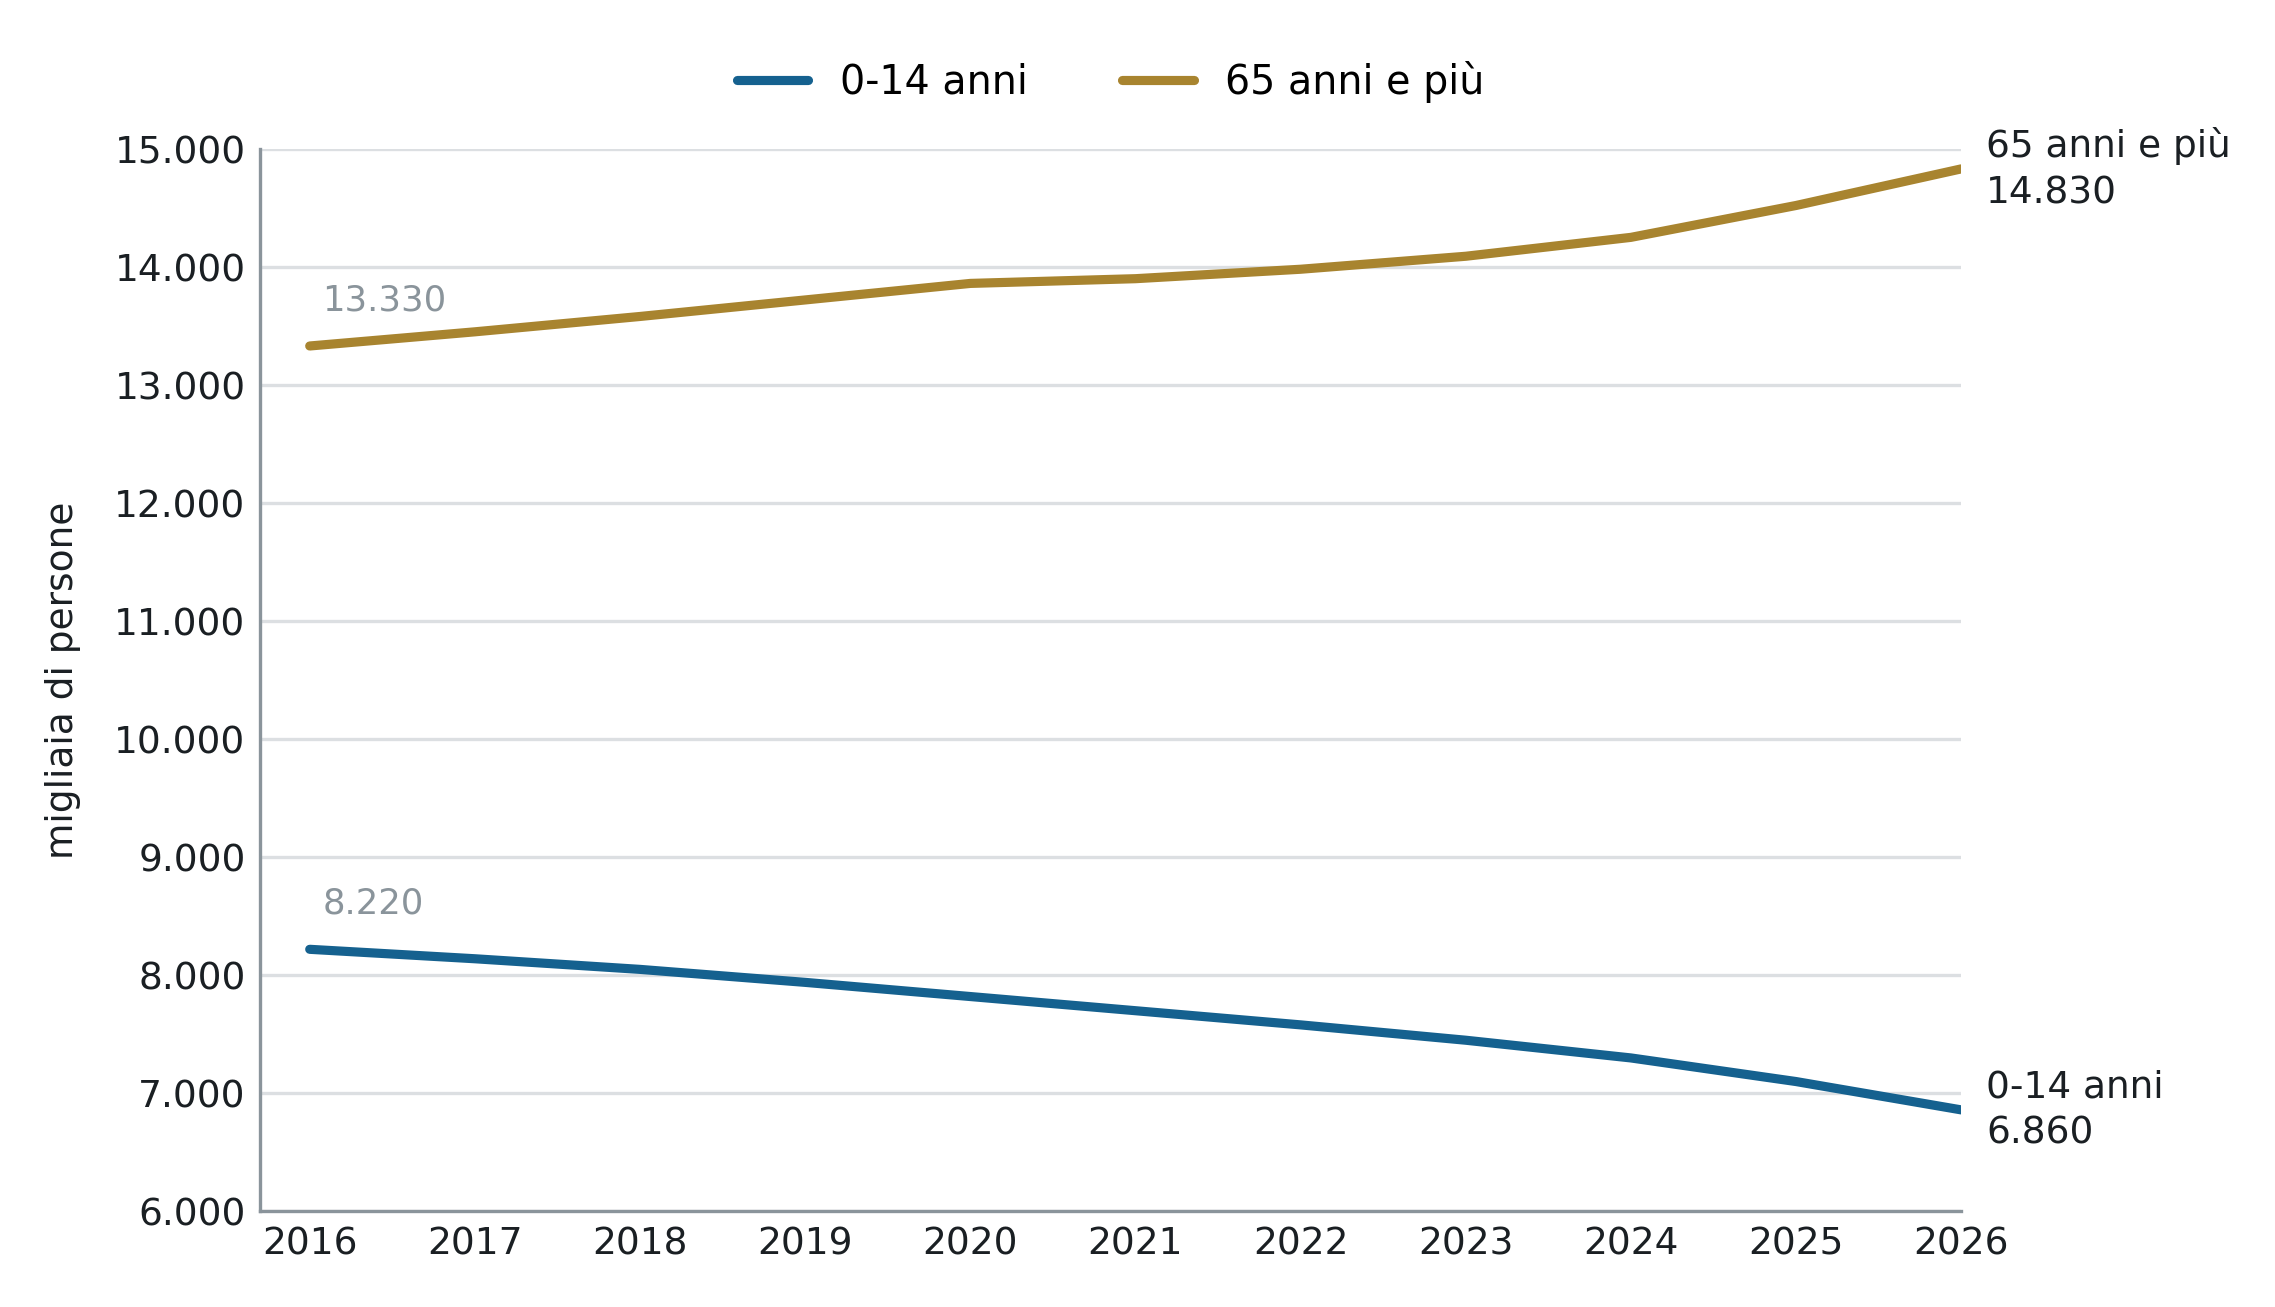
\includegraphics[width=0.85\linewidth]{figure/fig_popolazione.png}
    \caption{Italian population in the age bands 0-14 and 65 years and over,
    2016-2026.}
    \label{fig:popolazione}
\end{figure}

\subsection{Falls in the domestic environment and consequences for the person}

In a fall detection system it is not sufficient to know how often a person
falls; it is also necessary to consider where the event takes place and how
quickly it can be detected. Falls among people over sixty-five occur predominantly in the domestic environment: about 54\% take place at home, against 21\% in the garden, 20\% in the street and the remaining 5\% elsewhere \cite{PA}.

Falls are frequent in hospitals and care facilities as well. In that context,
however, the presence of staff generally makes it more likely that the event
is observed and that help arrives quickly. At home, by contrast, that
supervision is absent: the older person may remain on the ground for a much
longer time before anyone notices the fall, and particularly so if they live
alone.
The value of automatic detection is therefore greatest where human
supervision is absent. This does not rule out use in hospitals or in
residential care facilities, since a system of this kind remains useful for
reducing intervention times; but it explains why the domestic case is the one
on which the present work concentrates, and where it was experimentally
validated.

It is important to stress that the consequences of a fall do not depend on
the initial traumatic event alone. As reported in \cite{PA}, about 18\% of
falls caused a fracture and 16\% of falls required a hospital stay of at least
one day. Among hospital admissions for domestic accidents in the older
population, the most frequent diagnosis is hip fracture. Moreover, there
remains the problem of lying on the ground, which can favour secondary
complications such as dehydration, hypothermia, muscle damage and a general
worsening of the clinical condition.

Falls may also have psychological and functional consequences, including fear of falling, reduced confidence and the voluntary restriction of normal daily activities. Reducing the time between the fall and the arrival of help therefore does not serve only to limit the immediate damage: it is essential in order to guarantee a sustainable life in one's own home.

\section{Requirements of an automatic fall detection system}

A system intended for the detection of falls in a domestic or care
environment must satisfy requirements different from those of a classifier
evaluated exclusively on offline datasets. Achieving good classification
performance is not enough for the model to be usable.

For a solution of this kind to be adoptable, it must first of all detect the
event within a sufficiently short time and, at the same time, limit the
number of false alarms. A system that detects falls correctly but produces
continual alerts during normal daily activities risks becoming of little use
and, over time, being ignored or switched off. It must moreover handle data in a way compatible with the privacy of the people being monitored. Finally, the computational cost and that of the hardware must remain sufficiently contained to make a real installation and continuous operation possible.

These conditions translate into three main requirements: the first concerns
the operational reliability of the system and includes both the ability to
detect a fall promptly and the ability to contain false alarms. These two
aspects cannot be considered separately because improving one may entail the
worsening of the other. The second requirement concerns the protection of
privacy, while the third concerns the computational and economic
sustainability of the solution.

For these requirements to be experimentally verifiable, it is useful to translate them into measurable quantities. Table \ref{tab:criteri_valutazione} shows this correspondence, specifying the section in which each quantity is subsequently reported and verified.

\begin{table}[htbp]
\centering
\caption{Criteria used to evaluate the system.}
\label{tab:criteri_valutazione}
\resizebox{\textwidth}{!}{
\begin{tabular}{lll}
\toprule
\textbf{Requirement} & \textbf{Corresponding evaluation quantity} & \textbf{Section} \\
\midrule
Timeliness & Detection latency & \ref{sec:latenza} \\
Reliability & Event recall / missed falls & \ref{sec:recall-campo} \\
Alarm sustainability & False alarms per hour & \ref{sec:falsi-allarmi} \\
Computational feasibility & FPS / latency / memory / temperature & \ref{sec:costo-computazionale} \\
Privacy & Information retained, stored or transmitted & \ref{sec:protocollo-campo} \\
Continuous operation & Uninterrupted operating time & \ref{sec:continuita} \\
\bottomrule
\end{tabular}
}
\end{table}

\subsection{Timeliness and the sustainability of the alarm load}

The first requirement concerns timeliness. As discussed in the previous
section, a person who is unable to get up after a fall may remain on the
ground for a prolonged period before receiving assistance. The system must
therefore be able to recognise the event and generate an alert within a
sufficiently short interval of time.

Timeliness cannot, however, be considered separately from the reliability of
the alarm. A continuously active system produces a large number of decisions,
and every false positive may require a check by a family member, by a
caregiver or by care staff. If these alerts become too frequent, the system
risks proving of little use in everyday operation, even when it manages to
recognise most falls correctly.

Therefore, in real applications the number of false alarms produced per unit
of time takes on particular importance. One of the quantitative figures
available in the literature comes from a study conducted on sixteen older
adults monitored by means of a worn accelerometer, over a total of about
15.500 hours of use, reporting a rate of \textbf{0,049 alarms per hour}
\cite{KA}.
However, this value cannot be compared with the one produced by a vision-based system, since the acquisition modalities and the possible causes of error are different. The figure can nonetheless be used above all as a reference for the order of magnitude.

It is important to distinguish between two levels of evaluation. The first focuses on individual time windows and analyses the behaviour of the classifier. The second, on the other hand, concerns the alarm events that the system generates during operation. Several consecutive positive windows may belong to the same episode and can therefore be grouped into a single alarm. For this reason, the false positive rate per window and the number of false alarms per hour represent two different aspects of the system. The former measures the errors produced in individual windows, whilst the latter indicates how many false alarms are actually generated over time.

Precisely because the evaluation of vision-based systems is carried out
predominantly on laboratory datasets, classification metrics alone, such as
precision, recall and F-score, are not sufficient. The behaviour of the system
during prolonged operation is therefore also considered, distinguishing the
performance of the classifier on the individual temporal windows from the
number of alarm events actually generated.

\subsection{Confidentiality and local processing}

The use of a camera inside a home introduces a second important requirement:
the protection of personal data. An ordinary RGB stream may contain
identifying information relating to the person, to the environment in which
they live and to the activities they are performing.

The system should therefore minimise the use, storage and transmission of such identifiable visual information, using the original images only when necessary. However, this does not automatically guarantee the anonymity of the data, as even representations derived from the person's pose or movement may retain individual characteristics.

This choice reduces both the amount of identifiable visual information available to subsequent stages and the dimensionality of the data supplied to the classifier. Processing is moreover kept locally on the device, so that the video stream need not be transmitted to an external server. Only the data necessary for handling a possible alarm are sent outside.
This requirement motivates the pose-based, locally processed architecture developed in Chapter \ref{cap:metodologia}. 

\subsection{Cost, resources and edge architecture}

The choice to perform processing locally imposes a constraint on the available computational resources. A system intended to be installed permanently in a home or in a care facility should be able to run on compact, low-cost hardware, without necessarily depending on a workstation or on a remote computing infrastructure. Feasibility on the \emph{edge} device does not depend on the classifier alone. 

The computational cost should be assessed by considering data acquisition, pose estimation, feature extraction and classification together. 
It is thus necessary to strike a balance between recognition capability, computational complexity, latency and the ability to keep the entire pipeline running over time. This requirement leads to the adoption of an \emph{edge} architecture, the computational feasibility of which is verified experimentally in Chapter \ref{cap:edge}.

\section{Critical issues in the transfer from controlled data to the real
environment}

Evaluation on a controlled dataset makes it possible to compare
representations and models reproducibly, but it does not guarantee that the
system will maintain the same behaviour once installed in a real environment.

During the collection of a dataset many conditions are known or
controlled: the position of the cameras, the activities performed by the
subjects, the duration of the recordings and, in general, the context in which
acquisition takes place. In a real home these conditions may instead vary over
time.
In the case of a system based on pose estimation, three aspects prove
particularly important:
\begin{enumerate}
    \item the change of domain and of recording geometry,
    \item the presence of occlusions,
    \item the different frequency with which a fall occurs compared with
          normal daily activities.
\end{enumerate}

\subsection{Domain variation and recording geometry}

A first critical issue is the change in acquisition conditions. The
representation obtained from the pose estimator depends not only on
the movement performed by the person, but also on the way in which this
movement is observed by the camera.

The same action may appear different when observed from the front, from the
side or from a more elevated position. As a consequence, quantities derived
from the landmarks as well, such as trunk inclination, the displacements of
the various parts of the body or their apparent velocities, may take on
different values while describing the same movement.
The viewpoint then becomes a real problem for a system installed in
environments different from the one in which the training data were collected.
To this are added other variations, such as lighting, distance from the
camera, background, frame rate and the physical characteristics of the
observed subjects. 


Taken together, these differences produce a \emph{domain shift}, that is, a variation in the distribution of the data with respect to the one used in training. This problem has been divided into five categories, each associated with a specific experimental test as shown in Table \ref{tab:domain_shift}.

\begin{table}[htbp]
\centering
\caption{Types of domain shift considered.}
\label{tab:domain_shift}

\begin{tabularx}{\textwidth}{l X c}
\toprule
\textbf{Category} &
\textbf{Change considered} &
\textbf{Section} \\
\midrule
\emph{subject domain}
& change the subject observed
& \ref{sec:loso} \\
\emph{viewpoint shift}
& change the position of the camera with respect to the person
& \ref{sec:viewpoint} \\
\emph{frame-rate shift}
& change the acquisition rate
& \ref{sec:framerate} \\
\emph{dataset shift}
& change the dataset used
& \ref{sec:domainshift} \\
\emph{environment shift}
& change the capture environment
& \ref{sec:campo} \\
\bottomrule
\end{tabularx}
\end{table}

The performance obtained on the source domain is not
sufficient, on its own, to describe the generalisation capability of the system. For this reason, the different forms of domain shift are evaluated separately in the subsequent experiments.

\subsection{Occlusions and the quality of pose estimation}

A second critical issue concerns the visibility of the body.
In datasets collected under controlled conditions the subject is generally
filmed so as to be clearly visible. In a domestic or care environment, by
contrast, the person may be partly hidden by beds, chairs, tables or other
items of furniture. Occlusion may moreover occur during a fall itself, when
the body changes configuration rapidly or approaches the floor.

Under such conditions, the pose estimator may supply unstable coordinates or
fail to localise some landmarks correctly.
The problem weighs more here than elsewhere, because the features used by the
classifier are built precisely from the coordinates of the skeleton. An error
in the estimate of a landmark may therefore propagate to the geometric and
temporal quantities computed in the subsequent stages.
In Chapter~\ref{cap:sperimentale} the sensitivity to a partial loss of
information is studied through controlled tests in which some groups of
landmarks are made temporarily unavailable.

\subsection{Event prevalence and the base rate of false alarms}

A last difference between an experimental dataset and real operation concerns
the \emph{prevalence of the positive class}, that is, the frequency with which falls actually occur.

A dataset useful for training must contain a sufficient number of positive
examples, and the resulting percentage of falls is much higher than the one a
system encounters in operation, where almost all observations belong to normal
daily activities. The imbalance changes the weight that has to be attributed to
false positives.
Even a false-positive probability of $10^{-3}$ per decision may become operationally relevant if the system
produces several decisions per second over many hours of continuous monitoring.

It is nevertheless necessary to distinguish between positive windows and
actual alarm events. Within the same episode, the classifier may produce several consecutive windows, which the system's logic returns as a single alert.
It then becomes useful to consider two levels of reading:
\begin{itemize}
    \item [-] The first concerns the individual temporal windows and describes
          the behaviour of the classifier;
    \item [-] the second concerns the alarm events produced during continuous
          operation.
\end{itemize}
In the second case the measure that matters is the number of false alarms per
unit of time, because it represents the burden that the system imposes on the
user, on family members or on care staff. Chapter \ref{cap:edge} measures the ratio between the two counts and compares it with what was observed in the two homes.

\section{Definition of the event to be recognised}

Another aspect that needs to be clarified concerns the definition of the event that the system must detect.
A fall does not correspond to a single posture, but to an event that unfolds over time. Generally, the person starts from a stable position, goes through a phase of loss of balance and rapid change in posture, and then ends up on the ground or at a lower level.

From this temporal sequence, three phases can therefore be distinguished: the phase preceding the fall, the transition phase occurring during the fall, and the subsequent phase in which the subject is on the ground.
From a classification perspective, this phenomenon can be described in three different ways. One can identify the \emph{fall event}, which is the dynamic phase during which the body loses its balance and moves rapidly downwards; one can also identify the \emph{post-fall state}, when the person is already on the ground; or both conditions can be considered to trigger an alarm.

These definitions are closely related, but they are not equivalent. A person may still be in a low or lying position even during normal daily activities. Actions such as sitting down, kneeling or lying down intentionally can produce configurations similar to those observed after a fall. Therefore, the final posture alone may not be sufficient to distinguish between the two cases, leading to the consideration of the dynamics through which that posture is achieved. A fall is generally associated with an involuntary and rapid change in body configuration, whilst a voluntary movement tends to unfold more gradually.
Defining the positive class therefore amounts to a choice regarding the task required of the classifier, rather than a mere convention used during data labelling; this is because altering what is considered positive means changing the classification problem and, consequently, the type of errors the system may produce.

This chapter clarifies what is considered positive, specifying which events the system must recognise: the fall phase, the subsequent state, or both. The operational rule by which this choice is then transformed into the labels of the time windows is illustrated in Section \ref{sec:compito}, which is dedicated to the creation of the windows.

\section{Research questions and objectives}

In light of the above considerations, the aim of this work is to develop and evaluate a \emph{fall detection} system based on human motion analysis and designed to run locally on a low-cost \emph{edge} device. Starting from an RGB video, the system derives a skeletal representation by estimating the person's pose and uses geometric and temporal information to recognise a fall.

Interest is not, however, focused solely on achieving good performance on the development dataset, but also on understanding which aspects of the pipeline actually influence the system's behaviour and to what extent the results obtained under controlled conditions hold true as usage conditions vary.
Based on these objectives, three research questions were formulated:
\begin{description}
    \item[RQ1.] When movement representation and evaluation protocol are fixed, how strongly does classifier architecture affect fall-detection performance?
    \item[RQ2.] How much of the performance obtained under controlled conditions is preserved when subject, viewpoint, dataset and acquisition environment change?
    \item[RQ3.] Can the complete pose-based detection pipeline operate continuously on a low-cost edge device while maintaining acceptable latency and alarm load?
\end{description}

To answer these questions, this study is structured around four main directions:
\begin{enumerate}
    \item \textbf{Movement representation}: building, starting from the
          skeletal landmarks, compact and interpretable geometric and temporal
          representations of the movement of the body.
    \item \textbf{Temporal classification}: comparing different families of
          models on the same representation, in order to assess how far the
          choice of the classifier influences performance with respect to the
          other components of the pipeline.
    \item \textbf{Evaluation protocol}: analysing the effect of the main
          experimental choices, relating to the construction of the temporal
          windows, to labelling, to the separation of subjects between training
          and test and to the definition of the event to be recognised.
    \item \textbf{Deployment and transferability}: verifying that the entire
          pipeline can be executed continuously on an edge device and studying
          its behaviour as the subject, the viewpoint, the dataset and the
          acquisition environment vary. 
\end{enumerate}

The experimental section is structured around these research questions and progressively analyses how the system operates under the various conditions examined.